\begin{homeworkProblem}
\textbf{Optimal Policy for Simple MDP}

Consider the simple $n$-state MDP shown in Figure \ref{fig:optimal_policy}. Starting from state $s_1$, the agent can move to the right $(a_0)$ or left $(a_1)$ from any state $s_i$. Actions are deterministic and always succeed (e.g. going left from state $s_2$ goes to state $s_1$, and going left from state $s_1$ transitions to itself). Rewards are given upon taking an action from the state. Taking any action from the goal state $G$ earns a reward of $r=+1$ and the agent stays in state $G$. Otherwise, each move has zero reward $(r=0)$. Assume a discount factor $\gamma<1$.

\begin{figure}[h]
    \centering
    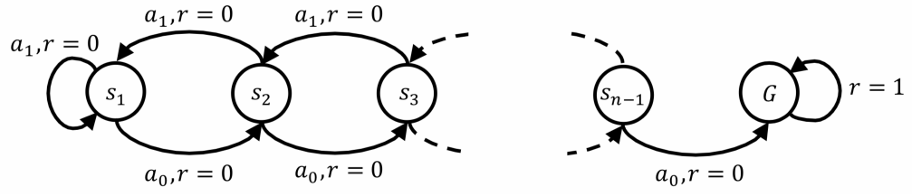
\includegraphics[width=0.8\textwidth]{./figure/optimal_policy.png}
    \caption{n-state MDP}
    \label{fig:optimal_policy}
\end{figure}

(a) The optimal action from any state $s_i$ is taking $a_0$ (right) until the agent reaches the goal state $G$. Find the optimal value function for all states $s_i$ and the goal state $G$.

(b) Does the optimal policy depend on the value of the discount factor $\gamma$? Explain your answer.

(c) Consider adding a constant $c$ to all rewards (i.e. taking any action from states $s_i$ has reward $c$ and any action from the goal state $G$ has reward $1+c$). Find the new optimal value function for all states $s_i$ and the goal state $G$. Does adding a constant reward $c$ change the optimal policy? Explain your answer.

(d) After adding a constant $c$ to all rewards now consider scaling all the rewards by a constant $a \left(\text{i.e.} r_{\text{new}}=a\left(c+r_{\text{old}}\right)\right)$. Find the new optimal value function for all states $s_i$ and the goal state $G$. Does that change the optimal policy? Explain your answer, If yes, give an example of $\alpha$ and $c$ that changes the optimal policy.

\solution

(a) Firstly, consider the state value function of $G$, since it has only one action:
\begin{align*}
v_*(G) &= \max_{a\in\A}\left(\R_G^a + \gamma\sum_{s'\in\mS}\mP_{G,s'}^av_*(s')\right) \\
&= 1 + \gamma v_*(G) \\
\Rightarrow v_*(G) &= \dfrac{1}{1-\gamma}
\end{align*}
Since the optimal policy is obvious, as it is given above, so we can get the state value function of all states using Bellman Optimality Equation. Define $G=s_{n}$, then $\forall i=1,2,\ldots,n-1$, we have:
\begin{align*}
v_*(s_i) &= \max_{a\in\A}\left(\R_{s_i}^a + \gamma\sum_{s'\in\mS}\mP_{s_i,s'}^av_*(s')\right) \\
&= 0 + \gamma \cdot 1 \cdot v_*(s_{i+1}) \\
&= \gamma v_*(s_{i+1})
\end{align*}
So above all, all states' value functions are:
\begin{align*}
v_*(G) &= \dfrac{1}{1-\gamma} \\
v_*(s_i) &= \dfrac{\gamma^{n-i}}{1-\gamma} \qquad \forall i=1,2,\ldots,n-1 \\
\end{align*}

(b) When $\gamma > 0$, the value of $\gamma$ does not change the relative order of the value functions of states, since
$$q_*(s,a)=\gamma v_*(s')$$
So the optimal policy will not change. i.e. $\forall i=1,\cdots,n-1, \pi(s_i) = a_0$.
However, when $\gamma = 0$, no matter what action($a_0$ or $a_1$) we take, the state-action value $q_*(s,a)$ will always be $0$, which are the same, so both $a_0$ and $a_1$ are the optimal actions.

(c) For any policy $\pi$, suppose the state value function is $v_{\pi}(s_i)$. If we fixed policy, but only change the reward, then the state value functions becomes $v_{\pi}'(s_i)$. Similarly, suppose the reward is $r_t'=r_t+c$. Then $\forall i=1,\cdots, n$, we have:
\begin{align*}
v_{\pi}'(s_i) &= \E_{\pi}[G_t|S_t=s_i] \\
&= \E_{\pi}\left[\sum_{t=0}^{\infty}r_t' \gamma^t|S_t=s_i\right] \\
&= \E_{\pi}\left[\sum_{t=0}^{\infty}(r_t+c) \gamma^t|S_t=s_i\right] \\
&= \E_{\pi}\left[\sum_{t=0}^{\infty}r_t \gamma^t|S_t=s_i\right] + \E_{\pi}\left[\sum_{t=0}^{\infty}c \gamma^t|S_t=s_i\right] \\
& = v_{\pi}(s_i) + \frac{c}{1-\gamma}
\end{align*}
Similarly,
$$q_{\pi}'(s,a)=\gamma v_{\pi}'(s')=\gamma v_{\pi}(s') + \frac{c\cdot \gamma}{1-\gamma}$$
Thus, the relative order of value functions of states will not change, and the optimal policy will not changed.

(d) Similarly with (c), but the new reward $r_t' = a(c+r_t)$, the value functions will be:
\begin{align*}
v_{\pi}'(s_i) &= \E_{\pi}[G_t|S_t=s_i] \\
&= \E_{\pi}\left[\sum_{t=0}^{\infty}r_t' \gamma^t|S_t=s_i\right] \\
&= \E_{\pi}\left[\sum_{t=0}^{\infty}a(r_t+c) \gamma^t|S_t=s_i\right] \\
&= a\cdot\E_{\pi}\left[\sum_{t=0}^{\infty}r_t \gamma^t|S_t=s_i\right] + a\cdot\E_{\pi}\left[\sum_{t=0}^{\infty}c \gamma^t|S_t=s_i\right] \\
& = a\cdot v_{\pi}(s_i) + \frac{ac}{1-\gamma}
\end{align*}
Similarly,
$$q_{\pi}'(s,a)=\gamma v_{\pi}'(s')=a\cdot\left(\gamma v_{\pi}(s') + \frac{c\cdot \gamma}{1-\gamma}\right)$$
So above all, if $a>0$, the relative order of $v(s_i)$ will not change, so the optimal policy will not change. \\
If $a=0$, then all states will have $q_*(s,a)=0$, so any policy is the optimal policy. \\
If $a<0$, then reaching $G$ would have the worst reward, so the optimal policy is to never reach $G$.

\end{homeworkProblem}

\newpage